\documentclass{article}
%\usepackage{fullpage}
\usepackage{sidecap}
\usepackage{mathtools}
\usepackage{mhchem}
\usepackage{amssymb}
\usepackage{amsmath}
\usepackage{bm}
\usepackage{gensymb}
\usepackage{siunitx}
\usepackage{cancel}
\usepackage{graphicx}
\usepackage{subcaption}
\author{Mann, J}
\title{Day 7 Notes}
\date{September 17, 2015}
\renewcommand{\d}[0]{\mathrm{d}}
\newcommand{\pOne}[2]{\frac{\partial #1}{\partial #2}}
\renewcommand{\deg}[0]{\degree}
\newcommand{\pTwo}[2]{\frac{\partial^2 #1}{\partial #2^2}}
\newcommand{\dOne}[2]{\frac{\d #1}{\d #2}}
\newcommand{\dTwo}[2]{\frac{\d^2 #1}{\d #2^2}}
\newcommand{\diag}[1]{\bcancel{#1}}
\newcommand{\matr}[1]{\bm{#1}}
\newcommand{\note}[1]{%
	\vspace{\parsep}%
	\textit{\textbf{Note: }}#1 \newline\newline
	\vspace{\parsep}}

\graphicspath{{Day7NotesPics/}}
\begin{document}
\maketitle
\begin{section}{Problem Set 1}

	\begin{enumerate}
		\item Be careful with $\frac{\Delta f}{\Delta x}\approx f^\prime$. Numerical derivatives of data can be really bad.
		\item Think about $\Gamma$ as $\Gamma [=] \frac{\text{molecules}}{(\text{nanometer})^2}$ or $\frac{1}{\Gamma} = A [=] \frac{(\text{nanometer})^2}{\text{molecules}}$, (in order to do this, you should use $k_B$ instead of $R$ (Boltzmann's constant instead of the ideal gas constant)
		\item Inverting Power Series.
		\item QUESTIONS: ``Some Details on least squares?''
	\end{enumerate}
\end{section}
\begin{section}{Some Details on Least Squares}
	\begin{subsection}{General Least squares analysis}
	\begin{align*}
		\Lambda_n &\equiv \text{Weight factor. This is used to place an amount of confidence on your data.}\\
		y_n &\equiv \text{Measured dependent variable data point}\\
		x_n &\equiv \text{Measured independent variable data point}\\
		\text{Sum}(\vec{\alpha}) &= \sum_{n=1}^{N}\Lambda_n (y_n - f(\vec{\alpha},x_n))^2
	\end{align*}
	This was developed by Gauss, and the data is assumed to follow a Gaussian distribution function it its errors.
	\begin{align*}
		\epsilon(x) &\equiv \text{A Gaussian distribution with mean: }\mu= 0\\
		y &= f(\vec{\alpha},x) + \epsilon(x)\\
		\text{now }\Lambda_n &= \left(\frac{\sigma}{\sigma_n}\right)^2
	\end{align*}
	Where $\sigma$ is the standard deviation, and $\sigma_n$ is the standard deviation of $y_n$.

	The fit is done so that the variation $\delta\text{sum} = 0$. Compute on $\alpha_1,\alpha_2,\ldots$.
	\begin{align*}
		0 = \delta(\text{Sum}(\alpha)) = \sum_{n=1}\Lambda_n \delta(y_n - f(\vec{\alpha},x_n))^2
	\end{align*}
	This generates a matrix problem. Expand $f(\vec{\alpha},x_n)$ in a Taylor's series keeping only the 1st order term in. $\Delta\vec{\alpha} = \vec{\alpha} - \alpha_0$.
	(Exchange $\sum\limits_n$ and sum over $\alpha_1, \alpha_2,\ldots$)
\begin{subsection}{Suppose you plot Sum vs $\vec{\alpha}$}
	\begin{figure}[h]
		\centering
		\begin{subfigure}[b]{0.4\textwidth}
		\centering
		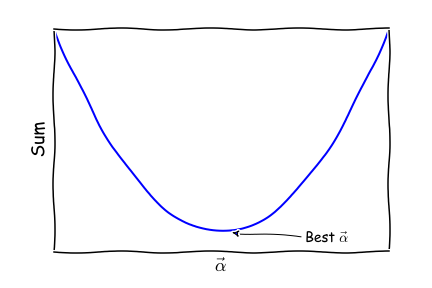
\includegraphics[height=100pt]{singleMinimum}
		\end{subfigure}
		\begin{subfigure}[b]{0.4\textwidth}
			\centering
			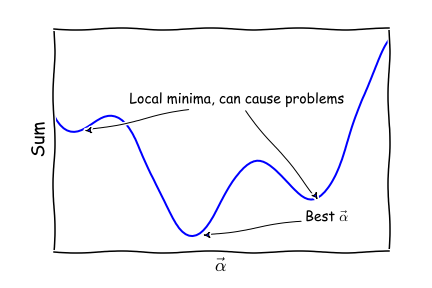
\includegraphics[height=100pt]{multipleMinima}
		\end{subfigure}
		\caption{A plot of two different error functions with respect to the sum. Note that this is oversimplified. Because $\vec{\alpha}$ is a vector, this will most often be an $n$-dimensional plot.}
		\label{fig:plots}
	\end{figure}
	If you are not careful, you may find the \underline{wrong minimum} in some cases. For example, consider Figure~\ref{fig:plots}
\end{subsection}
\begin{subsection}{Matrix approach}
	The result of $\delta\text{Sum} = 0$ is a matrix problem:
	\begin{align*}
		M_{ij}&=\sum_{n=1}^{N}\Lambda_n \pOne{f}{\alpha^i}\pOne{f}{\alpha^j}|_{x_n,\vec{\alpha_0}}\\
		\Delta \vec{\alpha} &= \vec{\alpha} - \alpha_0\\
		\matr{M}\Delta \vec{\alpha} &= \vec{R}
	\end{align*}
	This is the product matrix, some people call it the Hessian matrix.
	\note{A couple of properties to remember:
		\begin{align*}
			M_{ij} &= M_{ji}\\
			\det{(\matr{M})} &\neq 0
		\end{align*}
		This will be true when the ratio of $\frac{\text{maximum Eigenvalue}}{\text{minimum Eigenvalue}}$ is small enough.}
\end{subsection}

	\begin{align*}
		R_i &= \sum_{n=1}^{N}\Lambda_n(y_n - f(\vec{\alpha},x_n))\pOne{f}{\alpha_i}\Big|_{x,\alpha_0}\\
		\matr{M}\vec{\alpha}&=\vec{R}\\
		\vec{\alpha}&=\matr{M}^{-1}\vec{R}
	\end{align*}

	This is a matrix problem solved iteratively until $\delta\vec{\alpha} \rightarrow 0$, so we need a good $\vec{\alpha}_0$.

	For converged $\matr{M}$, 
	\begin{align*}
		(\matr{M}^{-1})_{ii} \rightarrow \sigma_{ii}^2\\
		\text{e.g.} (\matr{M}^{-1})_{11} = \sigma_{\alpha_1}^2
	\end{align*}
	Consider the Eigenvalue problem with $\matr{M}$, this gives you a set of Eigenvalues, one of which is a maximum, you divide that by the minimum eigenvalue, and you get the condition number, $c_N$.

	\begin{align*}
		c_N &\approx 1\text{, good fit}\\
		&\approx 10\text{ ok}\\
		&\approx 100\text{ ok}\\
		&\approx 10^4\text{ start being nervous}\\
		&> 10^5\text{ be \underline{very} careful}
	\end{align*}

	Plot the data! Plot the residuals ($y_n - f(\vec{\alpha},x_n)$)! The residuals plot should look random and centered around zero.
	\begin{figure}[h]
		\centering
		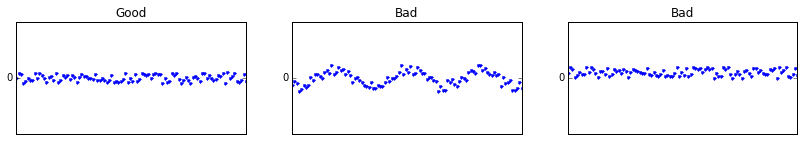
\includegraphics[height=60pt]{residuals}
		\caption{Three plots of the residuals. The first is good, the second shows correlation, and the third shows constant offset.}
		\label{fig:residuals}
	\end{figure}
\end{subsection}
\begin{subsection}{Summary}
	\begin{enumerate}
		\item The fit converges and the condition number is reasonable.
		\item Look at the residuals: Are they Gaussian? Plot them.
		\item Are the uncertainties of the parameters reasonable?
		\item The correlations are insignificant: 
			$\rho_{ij}$ is the correlation of parameter $\alpha_i$ with $\alpha_j$.
			\begin{align*}
				\rho_{ij} =	\frac{\matr{M}^{-1}}{\sqrt{(\matr{M}^{-1})_{ii}}\sqrt{(\matr{M}^{-1})_{jj}}}, -1\leq \rho_{ij} \leq 1
			\end{align*}



			\begin{itemize}
					\item $\rho_{ij} \approx 1$, $\alpha_i$ is a positive correlation with $\alpha_j$
					\item $\rho_{ij} \approx -1$, $\alpha_i$ is a negative correlation with $\alpha_j$
					\item $\rho_{ij} \in [-0.5,0.5]$, probably okay.
					\item $\rho_{ij} \not\in [-0.5,0.5]$, be very careful.
			\end{itemize}
	\end{enumerate}
	\note{If the fit is very good, then 
		\begin{align*}
			\frac{1}{N-P}\sum_{n=1}^{N}\Lambda_n(y_n - f(\vec{\alpha},x_n))^2 \rightarrow 1
		\end{align*}
	as the number of items, $N$, is large; $N\rightarrow \infty$. $P$ is the number of parameters. $N-P$ is the number of degrees of freedom for the fit.}
	\note{If the condition number is between 10 and 1000, your numerical inversion of $\matr{M}$ will be accurate. Start to be concerned if $c_N > 1000$, but $\matr{M}^{-1}$ may still be okay. $c_N > 10000$ shows that you should be concerned about the result. (This is from experience)}
\end{subsection}
\end{section}
\begin{section}{Notes about the homework}
	Temperature was in Kelvin. Using origin, there is a built-in algorithm for differentiation that is very nice.

	Analysis$\rightarrow$Mathematice$\rightarrow$Differentiate$\rightarrow$Open Dialog

	Choose the two columns that you will be using. There is a smoothing operation (it's pretty good). Look carefully at the pattern of your data, and make sure that it's smooth if it is supposed to be smooth.
	$\gamma = \gamma_{\circ} - kT\Gamma_\text{max}\ln{(1+ac)}$
Things to look for in a good fit:
\begin{itemize}
	\item The inverse hessian matrix (Look up the difference between Inverse Hessian and correlation matrix)
\end{itemize}
\end{section}
\begin{section}{XRC, X-Ray Crystallography}
	$1/\Gamma_\text{Max}$ is the surface area of the molecule.
NIH Has a crystallographic database that is useful in getting cross-sectional area of unit cells of a molecule, in case you need to use biological cells.

Suppose you need to know the concentration you need to put in a spray pesticide that is surface-active.

How would you get that?

Know what the molecule is, do an estimation of what the cross-sectional area of a molecule is as it goes into the interface, if it's long, get a piece of the molecule, then get geometric information about how it's going to pack.


\end{section}






\begin{section}{Inverting power series}

\end{section}











\end{document}
